%% Developing a solution for multimedia home networking chapter
%% author Liu Peng

We developed an Android application that has integrated with a simple media server, 
Airplay/DLNA/Chromecast device discovery, and Airplay/DLNA/Chromecast streaming
control point.

A simplified version of our implementation is shown in the figure \ref{chart3} below:
\begin{figure}[htb]
\centering 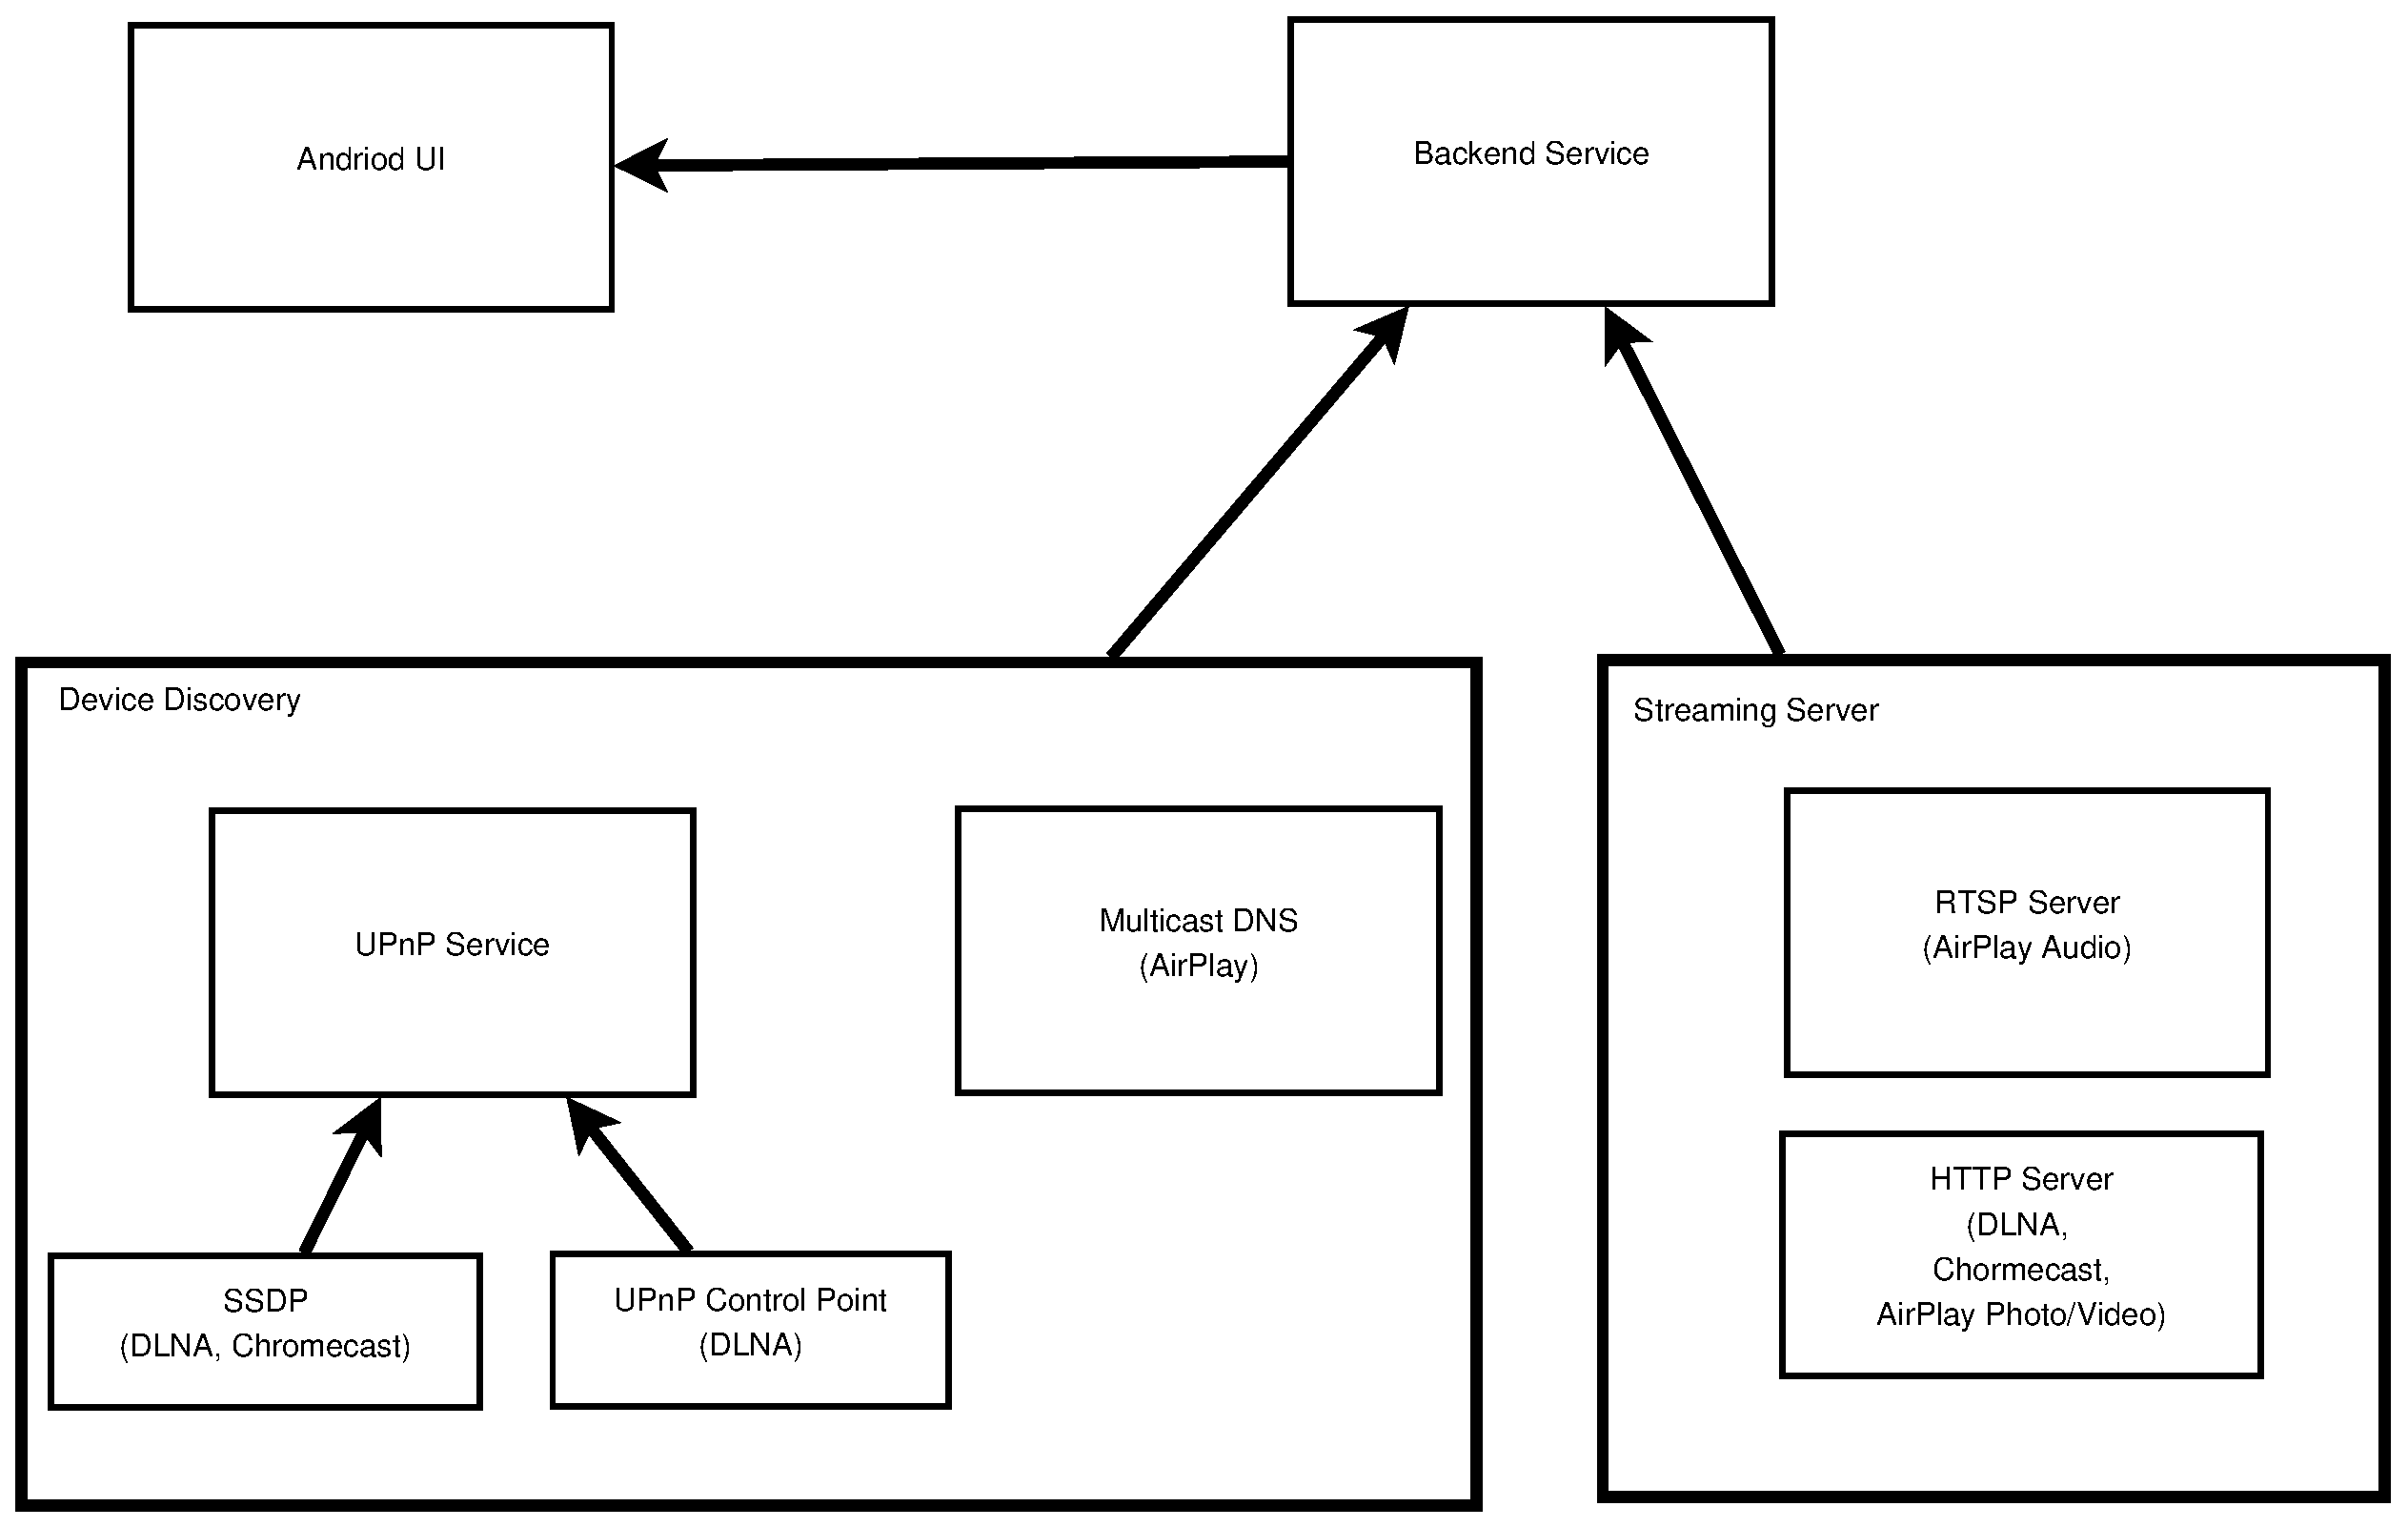
\includegraphics[height=9cm]{charts/chart3}
\caption{Simplified flow chart \label{chart3}}
\end{figure}

As we know that Airplay and DLNA works differently and have different features, but 
according to the previous study, we could combine some use cases of both protocols. 
We are developing an Android application that can handle most multimedia devices in 
a typical home networking. Feature list:

\begin{itemize}
\item[--]Firstly the app is a multimedia player, it can play music, photos and videos 
on SD card locally on Android phone
\item[--]It can stream local content to Apple TV, Airport express and Airplay-enabled 
speakers.
\item[--]It can stream local content to DLNA media renderers, which has a huge device 
base.
\item[--]It can stream local content to Chromecast devices.
\item[--]It can browse content from the DLNA media servers, a typical source is a 
Network Attached Storage (NAS). And play the media locally on the Android device.
\item[--]It can browse content from the DLNA media servers and stream it to DLNA media 
renderers.
\item[--]It can browse content from DLNA media servers and stream it to Airplay enabled 
devices using a different protocol.
\item[--]It can proxy online channels' content to DLNA and Airplay enabled devices. 
(Currently YouTube and Facebook videos are supported, but integration to Spotify is still 
in progress).
\end{itemize}